\documentclass[a4paper]{scrartcl}
\usepackage[ngerman]{babel}
\usepackage[utf8]{inputenc}
\usepackage[T1]{fontenc}
\usepackage{lmodern}
\usepackage{amssymb}
\usepackage{amsmath}
\usepackage{enumerate}
\usepackage{pgfplots}
\usepackage{scrpage2}\pagestyle{scrheadings}
\usepackage{tikz}
\usetikzlibrary{patterns}

\newcommand{\titleinfo}{Paralleliserungsschema}

\title{\titleinfo}
\author{Sönke Kracht, Sven-Hendrik Haase}
\date{\today}
\chead{\titleinfo}
\ohead{\today}
\setheadsepline{1pt}
\setcounter{secnumdepth}{0}
\newcommand{\qed}{\quad \square}

\begin{document}
\maketitle
\notag

\section{Jacobi-Verfahren}
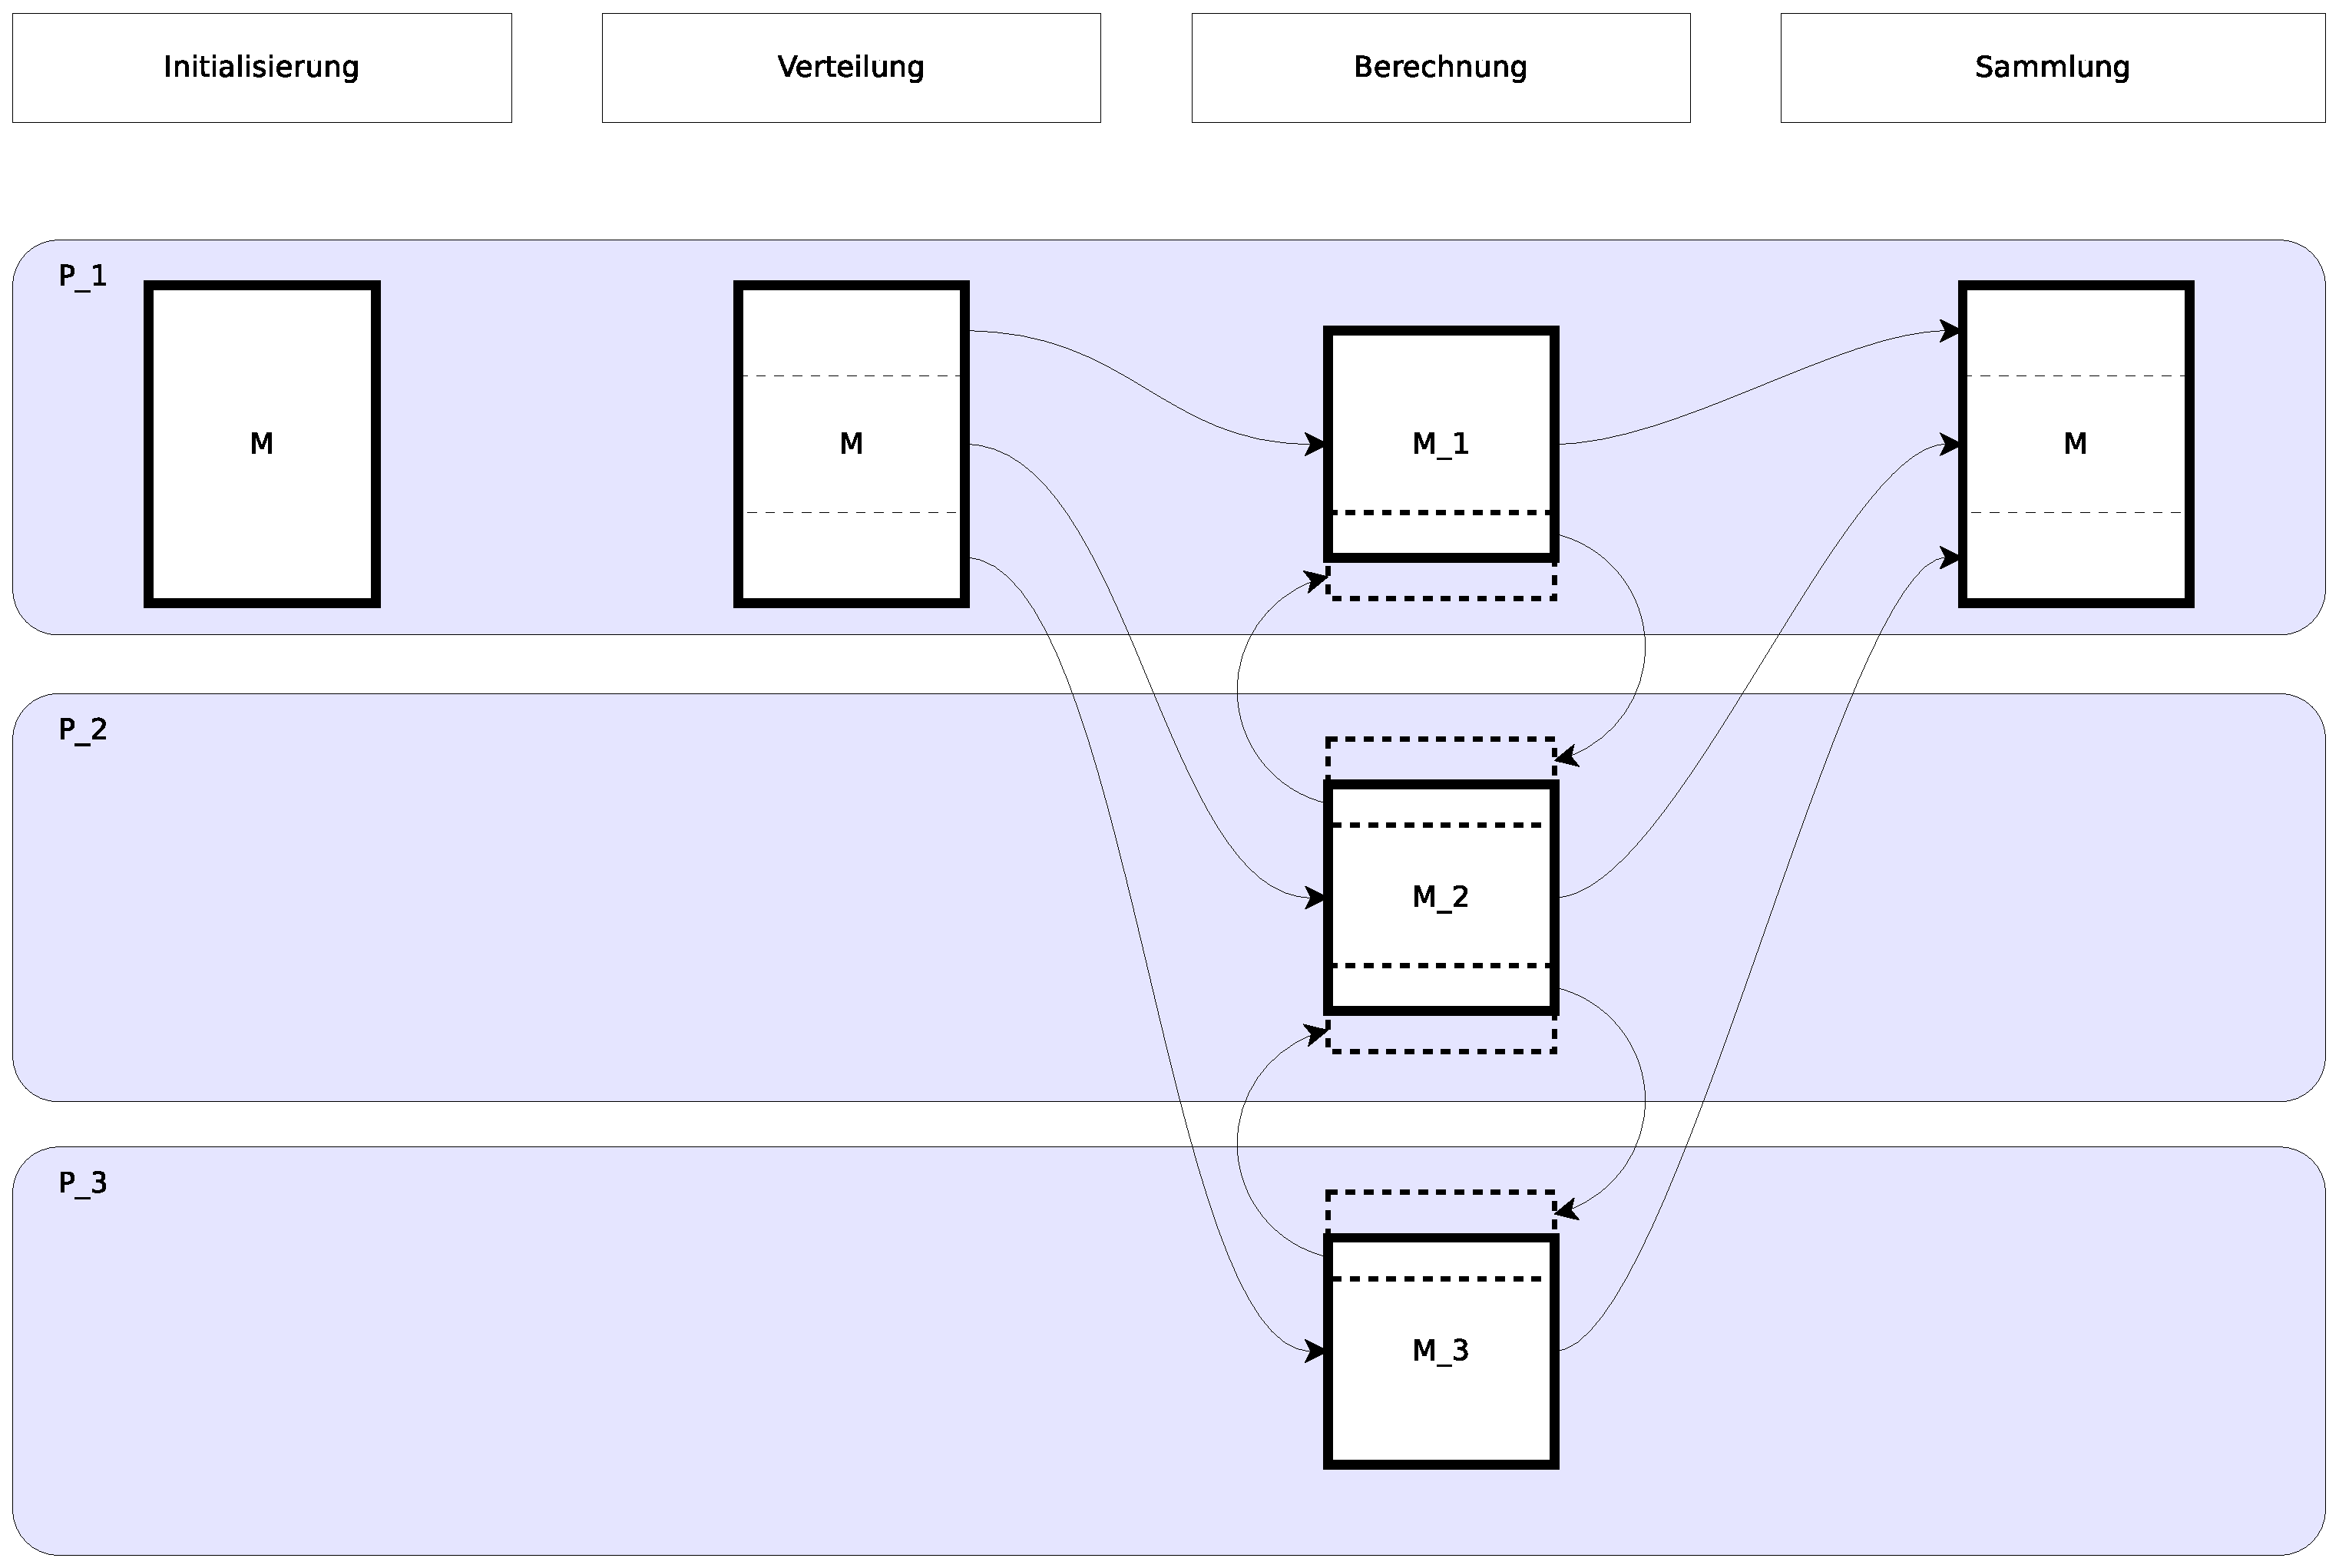
\includegraphics[scale=0.3]{Jacobi.eps}

\subsection{Aufteilung der Daten und Kommunikation}
Zu Beginn wird im Hauptprozess die gesamte Matrix initialisiert und auf die
Prozesse zu möglichst gleichen Teilen verteilt. Die Berechnung im Allgemeinen 
läuft innerhalb kleinerer Matrizen ab, die jeweils nur so groß sind, wie die 
Matrix, die er bei der Verteilung erhalten hat.
Jeder Prozess hat an seinen Matrixgrenzen je eine zusätzliche Zeile, über die
er mit seinen Nachbarprozessen kommuniziert. Ausnahmen hierbei sind natürlich
die Matrizen des ersten und des letzten Prozesses.\\
Eine Iteration läuft hierbei wie folgt ab:

Am Anfang der Iteration wird die Berechnung über die Inhalte der Matrix 
durchgführt. \\
Direkt nach der Berechnung sendet der Prozess asynchron an seine
Nachbarn die Zeilen, die diese für die nächste Iteration benötigen
(siehe Diagramm für Details). Beim Senden wird auch als MPI Tag die Zahl der
Iteration für diese Sendung übertragen.\\
Nach dem Senden wartet der Prozess auf 
die entsprechenden Daten seiner Nachbarn, damit er selbst mit der Berechnung 
der nächsten Iteration fortfahren kann.

Wenn die Abbruchbedingung erfüllt ist, senden alle Prozesse ihre Matrix an
den Hauptprozess, welcher die einzelnen kleinen Matrizen wieder zu einer großen
Marix zusammenfügt und das Programm beendet.

\subsection{Abbruchbedingungen}
\subsubsection{Iterativ}
Jeder Prozess hat einen Zähler, der sich die jeweilige Iteration speichert
und bei jeder Iteration um 1 dekrementiert. Wenn dieser Zähler 0 erreicht, wird
die Matrix wieder vom Hauptprozess zusammengesetzt.

\subsubsection{Genauigkeit}
Am Ende der Iteration wird vom Hauptprozess aus das maxresiduum aller Prozesse
per MPI\_Gather eingeholt und verglichen. Ist das maxresiduum aller Prozesse
kleiner als der maximale Fehler, ist die Abbruchbedingung erfüllt.

\newpage
\section{Gauss-Seidel-Verfahren}
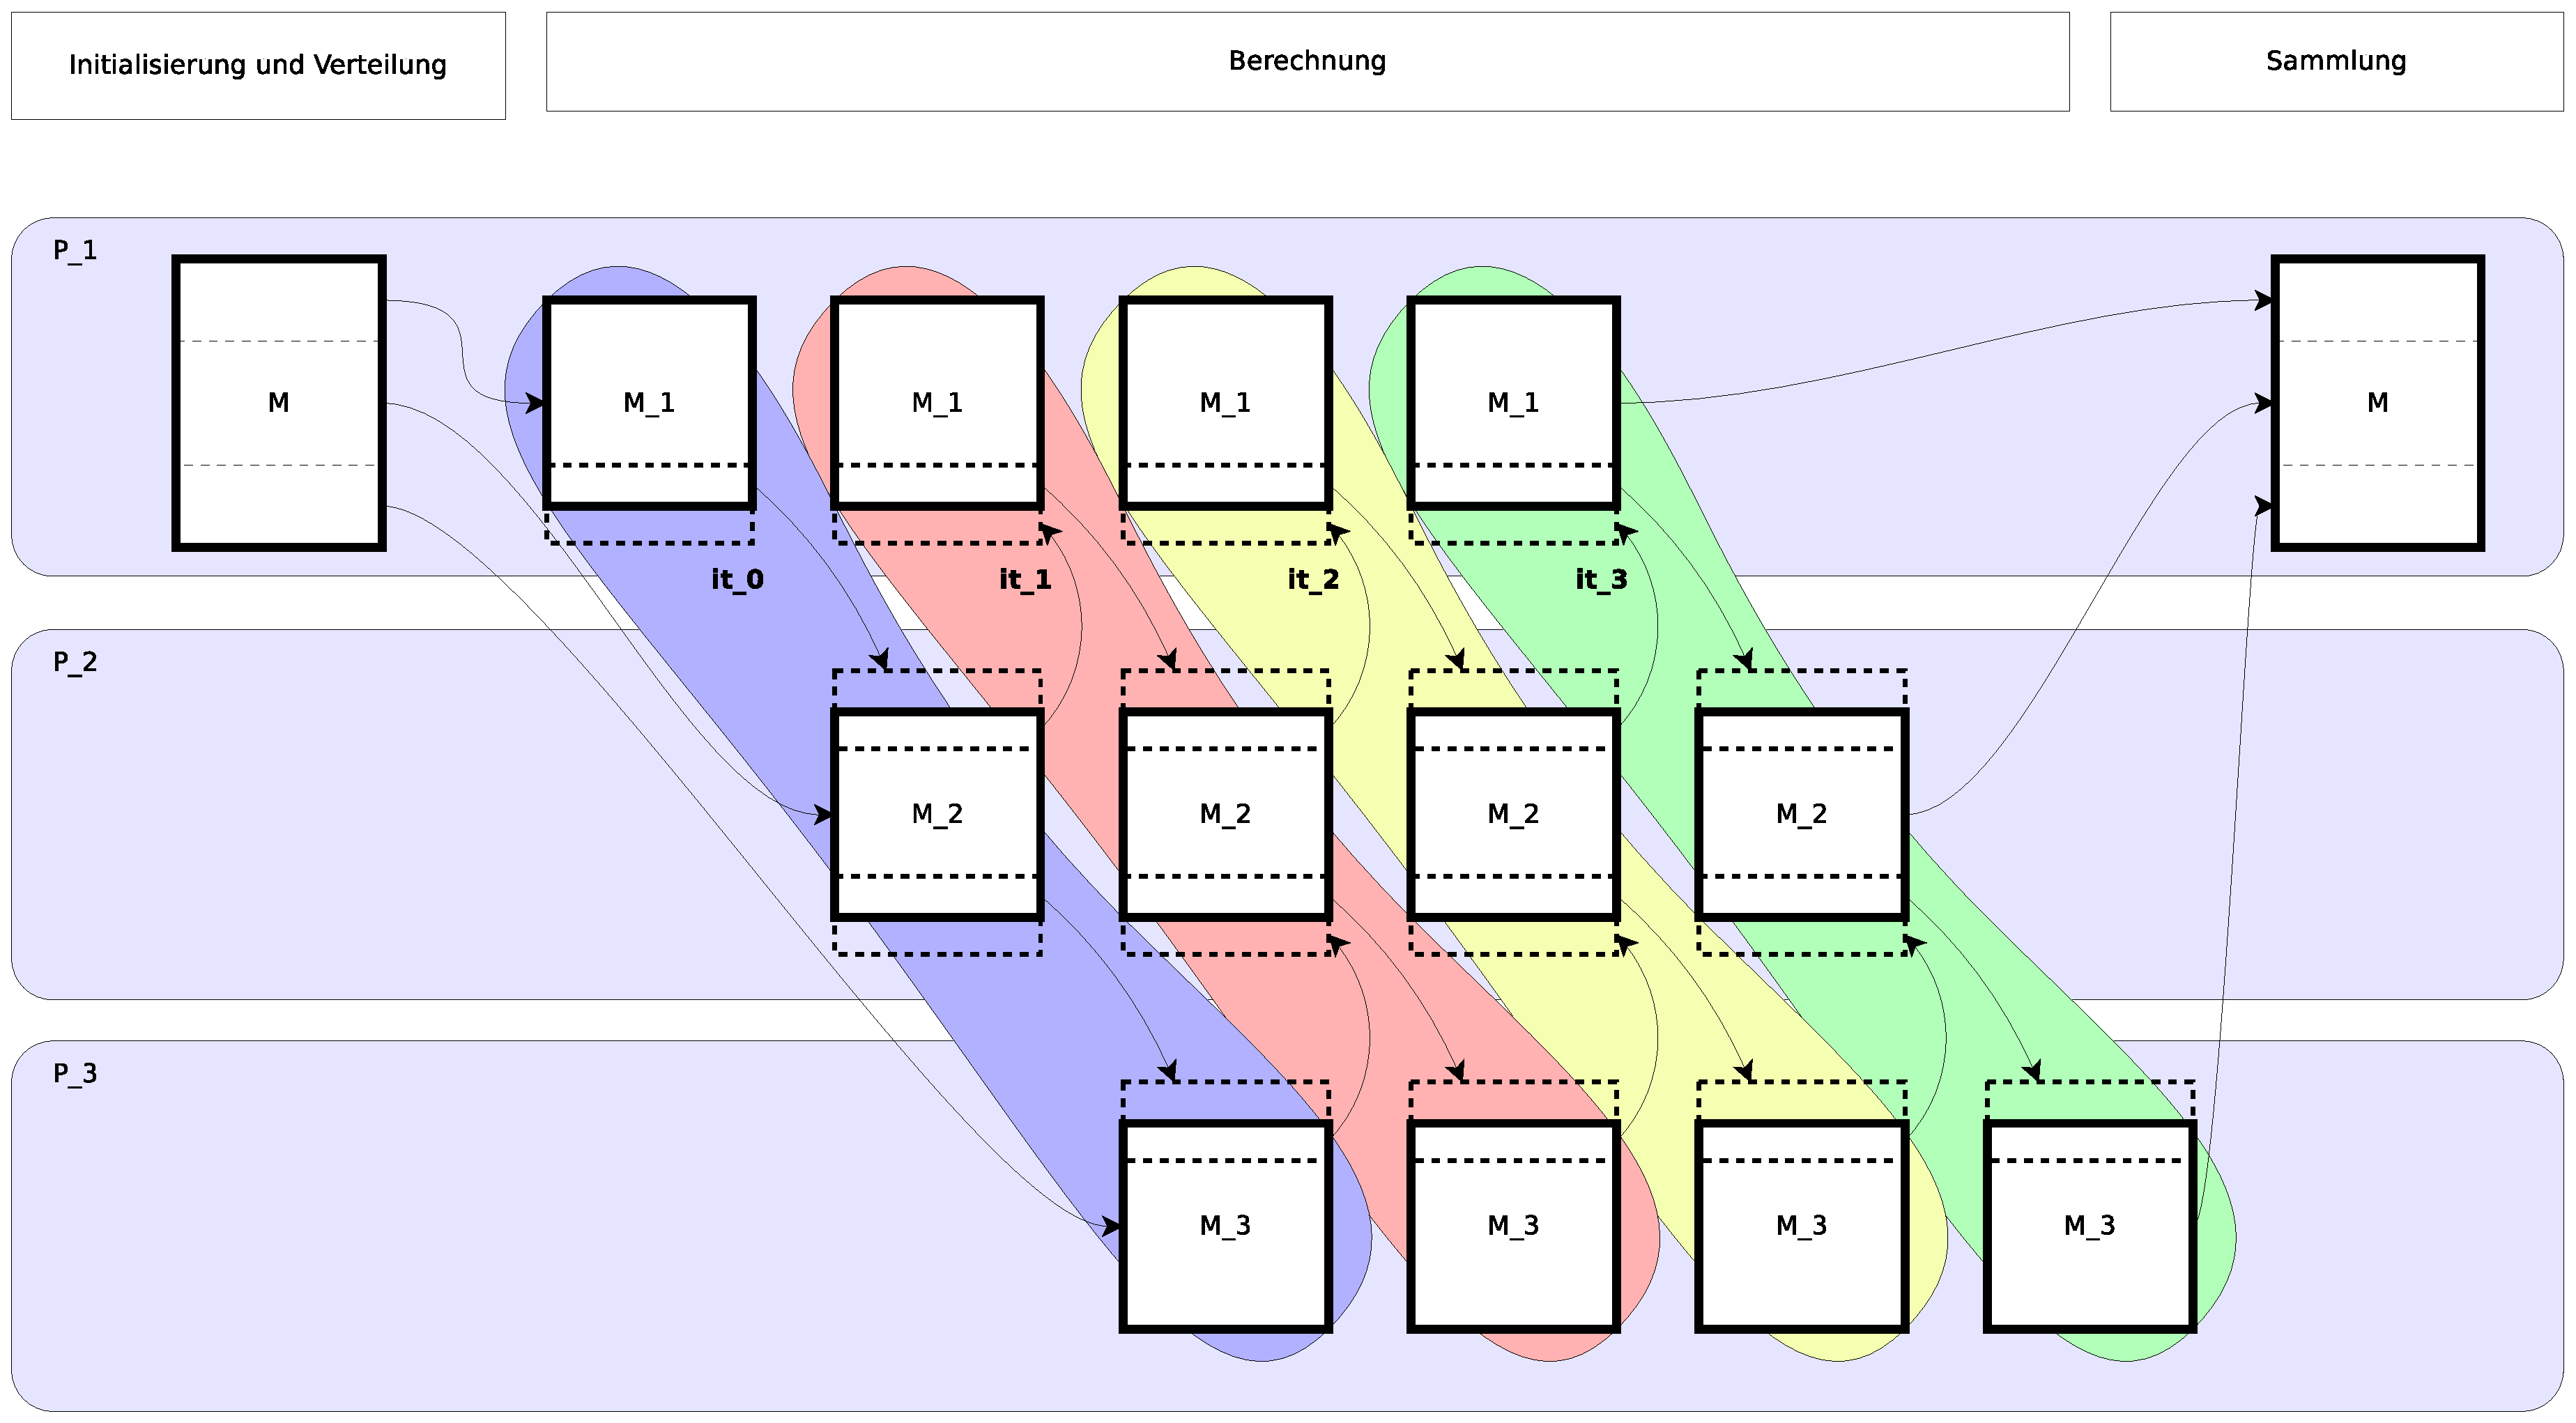
\includegraphics[scale=0.25]{GaussSeidel.eps}

\subsection{Aufteilung der Daten und Kommunikation}
Der Anfang verläuft ähnlich wie beim Jacobi-Verfahren samt Initialisierung
und Verteilung an die Unterprozesse. Auch hier gibt es eine zusätzliche
Zeile jenseits der eigenen Matrixgrenzen, die über MPI kommuniziert werden.\\
Eine Iteration läuft hierbei wie folgt ab:

Da jeder Wert von Werten abhängt, die in der selben Iteration berechnet werden
müssen, kann die Parallelität nicht trivial erfolgen wie beim Jacobi-Algorithmus.
Jede Iteration muss linear gerechnet werden, Parallelität kann nur durch das 
gleichzeitige Berechnen mehrerer aufeinanderfolgender Iterationen ereicht
werden. Dies wird mittels einer Pipeline realisiert.
Es ist hierbei zu bedenken, dass eine optimale Parallelität es erreicht wird,
wenn die Pipeline ''warm gelaufen'' ist. Das heißt, dass mindestens soviele
Iterationen wie Prozesse vorhanden sind. Während des Befüllens und Abbauens der
Pipeline geht unweigerlich Zeit verloren, weil die Prozesse auf Daten warten
müssen, die in diesem Verfahren leider nur nacheinander berechnet werden können.

Wenn die Abbruchbedingung erfüllt ist, senden alle Prozesse ihre Matrix an
den Hauptprozess, welcher die einzelnen kleinen Matrizen wieder zu einer großen
Marix zusammenfügt und das Programm beendet.

\subsection{Abbruchbedingungen}

\subsubsection{Iterativ}
Jeder Prozess kennt seine momentane Iteration und hält einfach sobald er 
fertig ist. Dadurch haben alle Prozesse am Ende eine Matrix in der 
gewünschten Iteration.

\subsubsection{Genauigkeit}
Da eine Iteration linear berechnet wird, kann die Abbruchbedingung auf
Genauigkeit erst im letzten Prozess überprüft werden. Zu diesem Zeitpunkt
befinden sich jedoch alle anderen Prozesse in späteren Iterationen. Das
bedeutet, dass man sich die alten Matrizen in den jeweiligen Prozessen merken
muss. Dabei müssen sich Prozesse mit kleinerem Rang mehr merken als Prozesse
höheren Ranges, weil sie sich noch nicht soweit von der Iteration des letzten 
Ranges entfernen konnten.

Jeder Vorgängerprozess muss sich eine Iteration 
mehr merken als sein Vorgänger. So kommt es zu einer Dreiecksstruktur beim 
Speicherbedarf. Konkret muss sich der höchste Prozess keine zusätzlichen 
Ergebnisse merken und der Prozess mit dem Rang 0 muss sich zusätzlich soviel 
alte Ergebnisse merken, dass er den Speicherbedarf der Gesamtmatrix hat.

Eine pragmatische Alternative hierzu wäre es, die Pipeline einfach auslaufen 
zu lassen. Dadurch spart man sich den zusätzlichen Speicher- und 
Verwaltungsaufwand, bekommt aber eine Matrix am Ende heraus, die sich streng 
genommen nicht in der gleichen Iteraton befindet. Dies ist aber kein 
praktisches Problem, da die Ergbnisse im Verlauf der Berechnungen sich nur 
verbessern. Abgesehen davon dürfte der Laufzeitverlust durch die 
Speicherverwaltung der streng korrekten Version den Zeitverlust, der durch 
das Auslaufen der Pipeline entsteht, mehr als ausgleichen.

\section{Rückmeldung}
Zeitaufwand: 5 Stunden\\
Lehrreich: Es war defintiv angemessen, sich mit dem Problem auseinander zu setzen, bevor man sich ans Programmieren macht.\\
Schwierigkeit: angemessen

\end{document}

